\section*{ИС К155ИР13}
\addcontentsline{toc}{section}{ИС К155ИР13}
\subsection*{Демонстрационная модель}
\addcontentsline{toc}{subsection}{Демонстрационная модель}

Универсальный сдвиговый регистр К155ИР13 является восьмиразрядным. Занесение
информации в регистр осуществляется в параллельном или последовательном коде.
Занесение информации в регистр выполняется по положительному перепаду. 
Считывание информации из регистра происходит в параллельном коде.

\begin{figure}[h!]
    \centering
    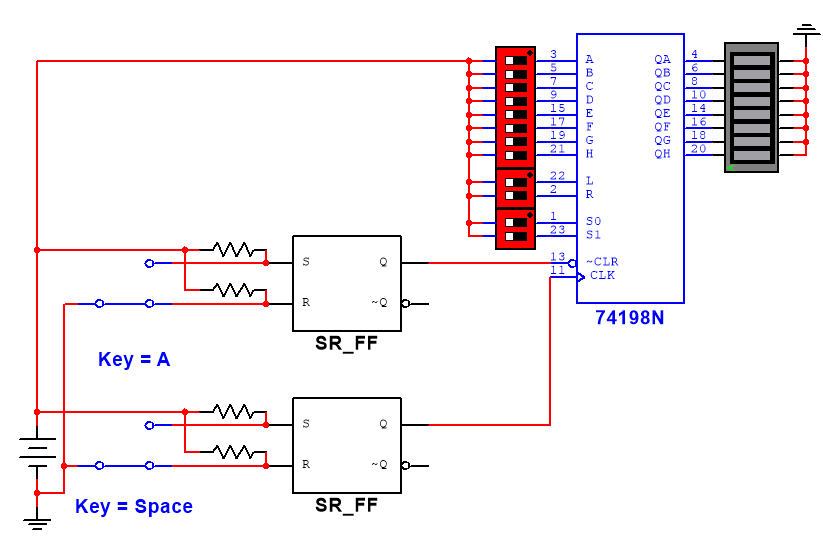
\includegraphics[scale=0.9]{images/image-2.png}
    \captionof{figure}{К155ИР13}
\end{figure}

\newpage

Далее схема была модифицирована таким образом, чтобы на базе ИС К155ИР13 был
получен универсальный кольцевой регистр. Для этого было учтено, что если
осуществляется сдвиг влево и на выходе A единица, то на выходе H должна будет появиться
единица. Аналогично, если осуществляется сдвиг вправо и на выходе H единица, то на
выходе A должна будет появиться единица. Ключи DL и DR в случае универсального
кольцевого регистра не нужны.

\begin{figure}[h!]
    \centering
    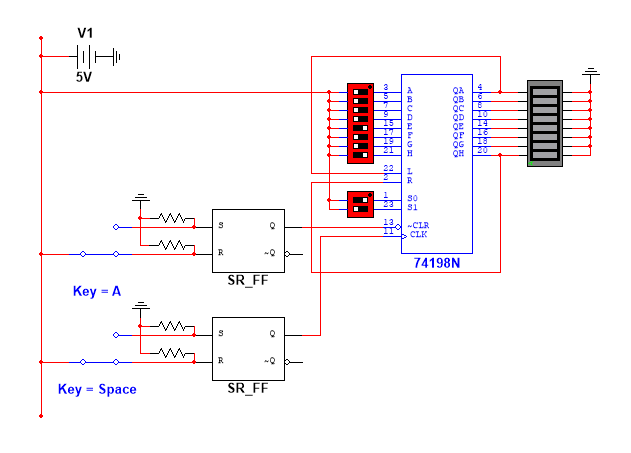
\includegraphics[scale=0.9]{images/image-3.png}
    \captionof{figure}{Универсальный кольцевой регистр}
\end{figure}